\section{顺反组}
\subsection{概述}
\begin{frame}
  \frametitle{顺反组 | \textcolor{red}{简介}}
  \begin{block}{维基百科}
顺反组(cistrome)指的是“全基因组尺度下反式作用因子的顺式作用靶点的集合,也可以说是在体情况下转录因子结合位点或组蛋白修饰在全基因组上的位置”。“顺反组”这一术语是cistron(顺反子)和genome(基因组)的混成词,最初由达纳-法伯癌症研究所和哈佛医学院的研究者命名。\\
\vspace{0.3em}
    染色质免疫沉淀等技术结合微阵列分析“ChIP-on-chip”或大规模并行DNA测序“ChIP-Seq”极大地方便了对转录因子及其它染色质相关蛋白的顺反组的定义。
  \end{block}
\end{frame}

\begin{frame}
  \frametitle{顺反组 | 简介}
  \begin{block}{Wikipedia}
    The cistrome refers to ``the set of cis-acting targets of a trans-acting factor on a genome-wide scale, also known as the \textit{in vivo} genome-wide location of transcription factor binding-sites or histone modifications". The term cistrome is a portmanteau of cistr (from cistron) + ome (from genome). The term cistrome was coined by investigators at the Dana-Farber Cancer Institute and Harvard Medical School.\\
\vspace{0.3em}
    Technologies such as chromatin immunoprecipitation combined with microarray analysis ``ChIP-on-chip" or with massively parallel DNA sequencing ``ChIP-Seq" have greatly facilitated the definition of the cistrome of transcription factors and other chromatin associated proteins.
  \end{block}
\end{frame}

\begin{frame}
  \frametitle{顺反组 | \textcolor{red}{简介}}
  \begin{block}{百度百科}
    顺反组(cistrome)是由“Dana-Farber癌症研究所”与哈佛医学院的科学家提出的遗传学术语,用于定义一个反式(trans)调控因子在基因组(genome)范围内的作用对象——一组顺式(cis)作用元素。一些技术,例如免疫共沉淀与基因芯片结合的技术(ChIP-on-chip),已经被广泛的应用于发现转录因子以及其他染色质相关因子的顺反组。
  \end{block}
\end{frame}

\begin{frame}
  \frametitle{顺反组 | 简介}
  \begin{figure}
    \centering
    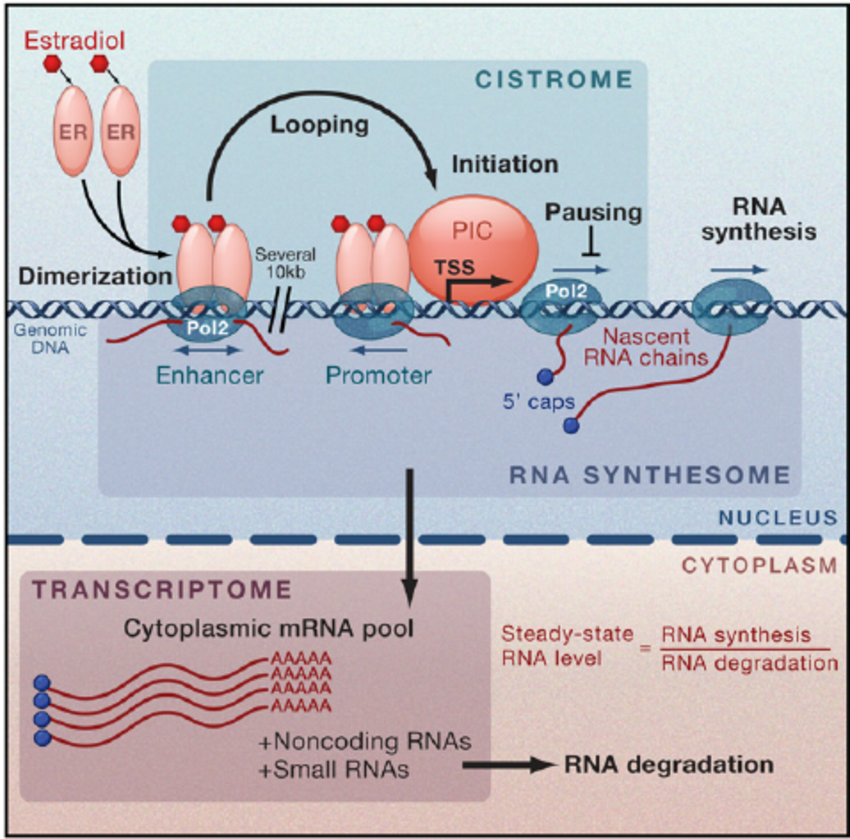
\includegraphics[width=0.65\textwidth]{c3.transcriptome/cistrome.01.png}
  \end{figure}
\end{frame}

\begin{frame}
  \frametitle{顺反组 | 研究方法 | ChIP-on-chip}
  \begin{block}{ChIP-on-chip}
    ChIP-on-chip (also known as ChIP-chip) is a technology that combines chromatin immunoprecipitation (``ChIP") with DNA microarray (``chip").\\
    \vspace{1em}
    Like regular ChIP, ChIP-on-chip is used to investigate \textcolor{red}{interactions between proteins and DNA} \textit{in vivo}. Specifically, it allows the identification of the cistrome, sum of binding sites, for DNA-binding proteins on a genome-wide basis. Whole-genome analysis can be performed to determine the locations of binding sites for almost any protein of interest. As the name of the technique suggests, such proteins are generally those operating in the context of chromatin. The most prominent representatives of this class are transcription factors, replication-related proteins, like Origin Recognition Complex Protein(ORC), histones, their variants, and histone modifications.
  \end{block}
\end{frame}

\begin{frame}
  \frametitle{顺反组 | 研究方法 | ChIP-on-chip}
  \begin{figure}
    \centering
    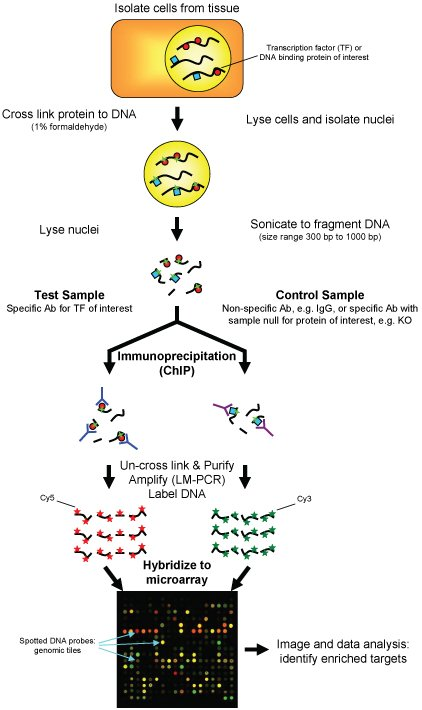
\includegraphics[width=0.4\textwidth]{c3.transcriptome/method.coc.01.jpg}
  \end{figure}
\end{frame}

\begin{frame}
  \frametitle{顺反组 | 研究方法 | ChIP-on-chip}
  \begin{figure}
    \centering
    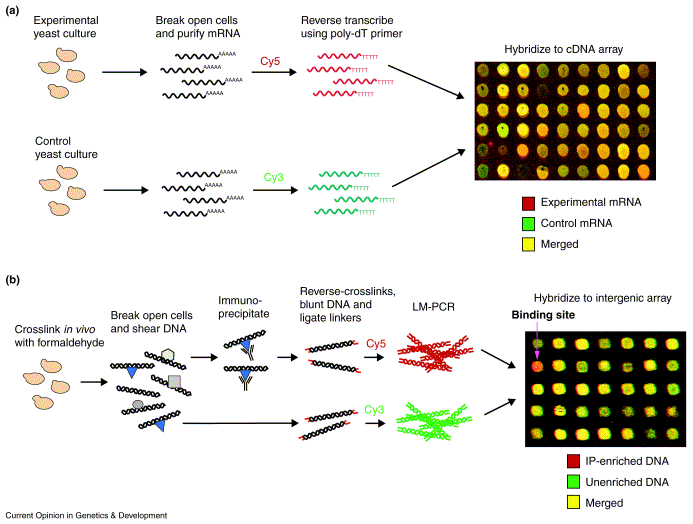
\includegraphics[width=0.8\textwidth]{c3.transcriptome/method.coc.04.png}
  \end{figure}
\end{frame}

\begin{frame}
  \frametitle{顺反组 | 研究方法 | ChIP-Seq}
  {\footnotesize
  \begin{block}{ChIP-Seq}
    染色质免疫沉淀-测序(ChIP-sequencing,简称为ChIP-seq)被用于分析\textcolor{red}{蛋白质与DNA的交互作用}。该技术将染色质免疫沉淀(ChIP)与大规模并行DNA测序结合起来以鉴定与DNA相关蛋白的结合部位。其可被用于精确绘制任意目的蛋白在全基因组上的结合位点。在此之前,ChIP-on-chip是研究这些蛋白-DNA联系的最常用的技术。
  \end{block}
  }
  \begin{figure}
    \centering
    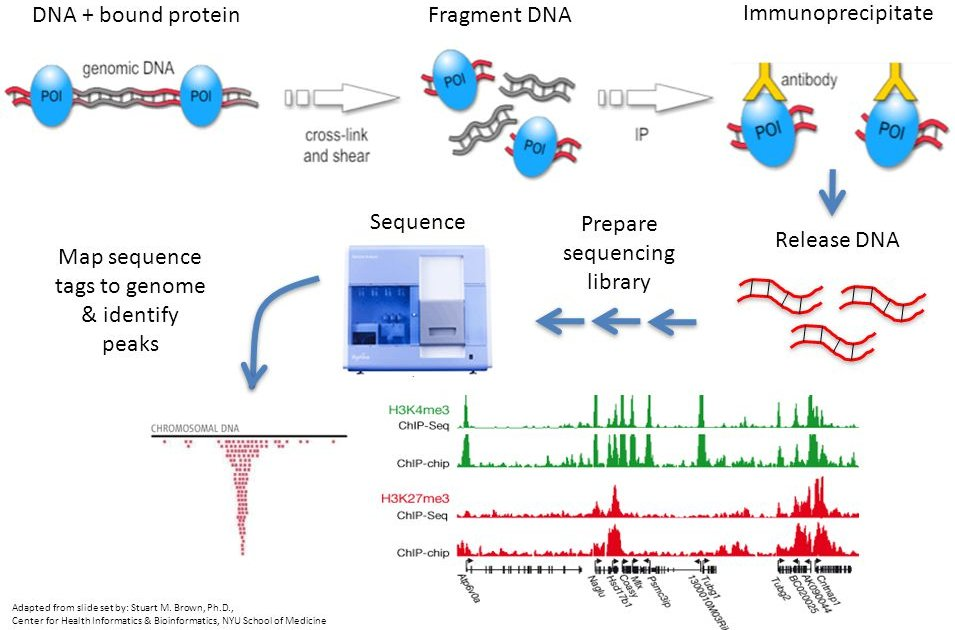
\includegraphics[width=0.65\textwidth]{c3.transcriptome/method.cs.01.jpg}
  \end{figure}
\end{frame}

\begin{frame}
  \frametitle{顺反组 | 研究方法 | ChIP-Seq vs. ChIP-chip}
  \begin{figure}
    \centering
    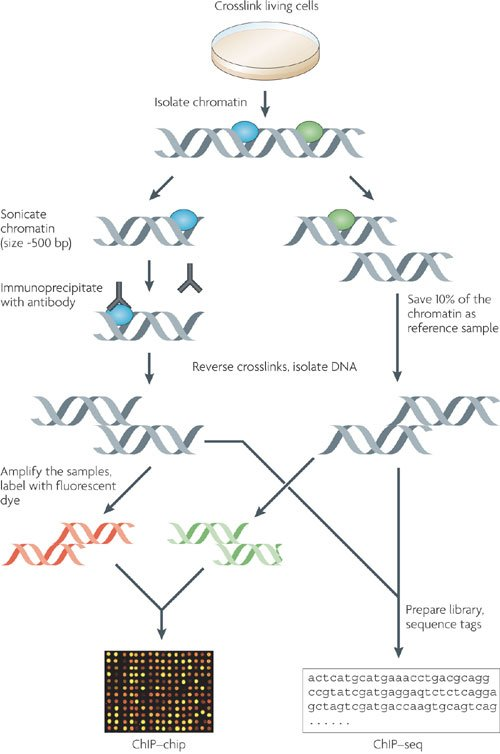
\includegraphics[width=0.43\textwidth]{c3.transcriptome/method.coc.cs.01.jpg}
  \end{figure}
\end{frame}

\subsection{ChIP-Seq}
\subsubsection{技术简介}
% \begin{frame}
%   \frametitle{顺反组 | \textcolor{red}{ChIP-Seq}}
%   \begin{block}{ChIP-Seq}
% 染色质免疫沉淀-测序(ChIP-sequencing,简称为ChIP-Seq)被用于分析蛋白质与DNA的交互作用。该技术将染色质免疫沉淀(ChIP)与大规模并行DNA测序结合起来以鉴定与DNA相关蛋白的结合部位。其可被用于精确绘制任意目的蛋白在全基因组上的结合位点。在此之前,ChIP-on-chip是研究这些蛋白-DNA联系的最常用的技术。
%   \end{block}
% \end{frame}

\begin{frame}
  \frametitle{顺反组 | 研究方法 | ChIP-Seq}
  {\footnotesize
  \begin{block}{ChIP-Seq}
    染色质免疫沉淀-测序(ChIP-sequencing,简称为ChIP-seq)被用于分析\textcolor{red}{蛋白质与DNA的交互作用}。该技术将染色质免疫沉淀(ChIP)与大规模并行DNA测序结合起来以鉴定与DNA相关蛋白的结合部位。其可被用于精确绘制任意目的蛋白在全基因组上的结合位点。在此之前,ChIP-on-chip是研究这些蛋白-DNA联系的最常用的技术。
  \end{block}
  }
  \begin{figure}
    \centering
    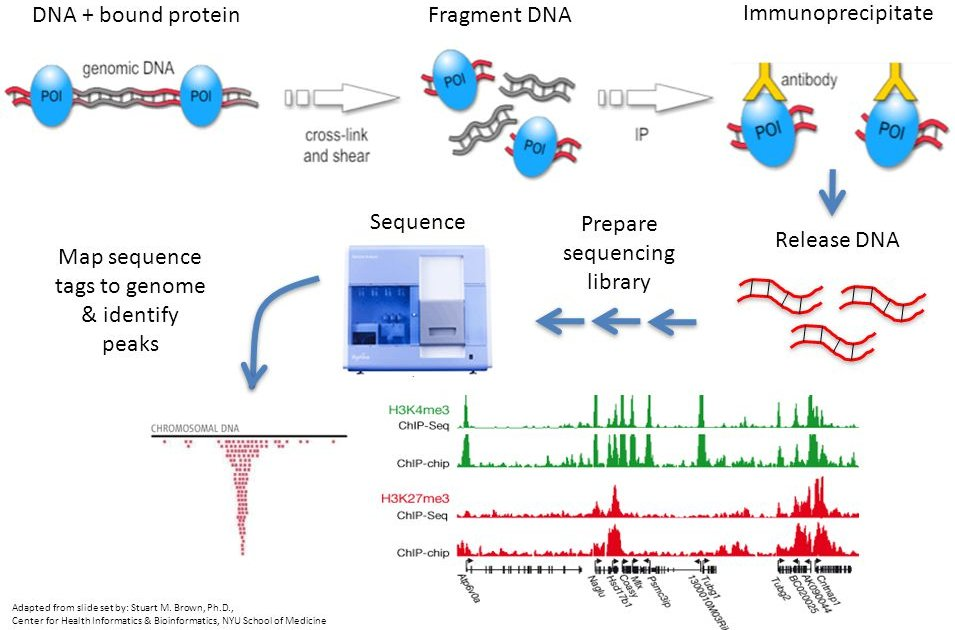
\includegraphics[width=0.65\textwidth]{c3.transcriptome/method.cs.01.jpg}
  \end{figure}
\end{frame}

\begin{frame}
  \frametitle{顺反组 | ChIP-Seq}
  \begin{block}{ChIP-Seq}
    ChIP-sequencing, also known as ChIP-seq, is a method used to analyze protein interactions with DNA. ChIP-seq combines chromatin immunoprecipitation (ChIP) with massively parallel DNA sequencing to identify the binding sites of DNA-associated proteins. It can be used to map global binding sites precisely for any protein of interest. Previously, ChIP-on-chip was the most common technique utilized to study these protein-DNA relations.
  \end{block}
\end{frame}

\begin{frame}
  \frametitle{顺反组 | ChIP-Seq | Uses}
  \begin{block}{Uses}
    ChIP-seq is used primarily to determine how transcription factors and other chromatin-associated proteins influence phenotype-affecting mechanisms. Determining how proteins interact with DNA to regulate gene expression is essential for fully understanding many biological processes and disease states. This epigenetic information is complementary to genotype and expression analysis.\\
    \vspace{1em}
    ChIP-seq technology is currently seen primarily as an alternative to ChIP-chip which requires a hybridization array. This necessarily introduces some bias, as an array is restricted to a fixed number of probes. Sequencing, by contrast, is thought to have less bias, although the sequencing bias of different sequencing technologies is not yet fully understood.\\
  \end{block}
\end{frame}

\begin{frame}
  \frametitle{顺反组 | ChIP-Seq | Uses}
  {\footnotesize
  \begin{block}{Uses}
    Specific DNA sites in direct physical interaction with transcription factors and other proteins can be isolated by chromatin immunoprecipitation. ChIP produces a library of target DNA sites bound to a protein of interest \textit{in vivo}.\\
    \vspace{1em}
    Massively parallel sequence analyses are used in conjunction with whole-genome sequence databases to analyze the interaction pattern of any protein with DNA, or the pattern of any epigenetic chromatin modifications. This can be applied to the set of ChIP-able proteins and modifications, such as transcription factors, polymerases and transcriptional machinery, structural proteins, protein modifications, and DNA modifications.\\
    \vspace{1em}
    As an alternative to the dependence on specific antibodies, different methods have been developed to find the superset of all nucleosome-depleted or nucleosome-disrupted active regulatory regions in the genome, like DNase-Seq and FAIRE-Seq.
  \end{block}
  }
\end{frame}

\begin{frame}
  \frametitle{顺反组 | ChIP-Seq | Workflow}
  \begin{block}{ChIP}
    ChIP is a powerful method to selectively enrich for DNA sequences bound by a particular protein in living cells. However, the widespread use of this method has been limited by the lack of a sufficiently robust method to identify all of the enriched DNA sequences. The ChIP process enriches specific crosslinked DNA-protein complexes using an antibody against the protein of interest. Oligonucleotide adaptors are then added to the small stretches of DNA that were bound to the protein of interest to enable massively parallel sequencing.
  \end{block}
\end{frame}

\begin{frame}
  \frametitle{顺反组 | ChIP-Seq | Workflow}
  \begin{block}{Sequencing}
    After size selection, all the resulting ChIP-DNA fragments are sequenced simultaneously using a genome sequencer. A single sequencing run can scan for genome-wide associations with high resolution, meaning that features can be located precisely on the chromosomes. ChIP-chip, by contrast, requires large sets of tiling arrays for lower resolution.\\
    \vspace{1em}
    There are many new sequencing methods used in this sequencing step. Then, the data collection and analysis software aligns sample sequences to a known genomic sequence to identify the ChIP-DNA fragments.
  \end{block}
\end{frame}

\begin{frame}
  \frametitle{顺反组 | ChIP-Seq | Sensitivity}
  \begin{block}{Sensitivity}
    Sensitivity of this technology depends on the depth of the sequencing run (i.e. the number of mapped sequence tags), the size of the genome and the distribution of the target factor. The sequencing depth is directly correlated with cost. If abundant binders in large genomes have to be mapped with high sensitivity, costs are high as an enormously high number of sequence tags will be required. This is in contrast to ChIP-chip in which the costs are not correlated with sensitivity.
  \end{block}
\end{frame}

\begin{frame}
  \frametitle{顺反组 | ChIP-Seq | Precision}
  \begin{block}{Precision}
    Unlike microarray-based ChIP methods, the precision of the ChIP-seq assay is not limited by the spacing of predetermined probes. By integrating a large number of short reads, highly precise binding site localization is obtained. Compared to ChIP-chip, ChIP-seq data can be used to locate the binding site within few tens of base pairs of the actual protein binding site. Tag densities at the binding sites are a good indicator of protein-DNA binding affinity, which makes it easier to quantify and compare binding affinities of a protein to different DNA sites.
  \end{block}
\end{frame}

\begin{frame}
  \frametitle{顺反组 | ChIP-Seq | Computational analysis}
  \begin{block}{Computational analysis}
    As with many high-throughput sequencing approaches, ChIP-seq generates extremely large data sets, for which appropriate computational analysis methods are required. To predict DNA-binding sites from ChIP-seq read count data, peak calling methods have been developed. The most popular method is MACS which empirically models the shift size of ChIP-Seq tags, and uses it to improve the spatial resolution of predicted binding sites.\\
    \vspace{1em}
    Another relevant computational problem is Differential peak calling, which identifies significant differences in two ChIP-seq signals from distinct biological conditions. Differential peak callers segment two ChIP-seq signals and identify differential peaks using Hidden Markov Models. Examples for two-stage differential peak callers are ChIPDiff and ODIN.
  \end{block}
\end{frame}

\subsubsection{数据分析}
\begin{frame}
  \frametitle{顺反组 | ChIP-Seq | 分析 | \textcolor{red}{流程}}
  \begin{figure}
    \centering
    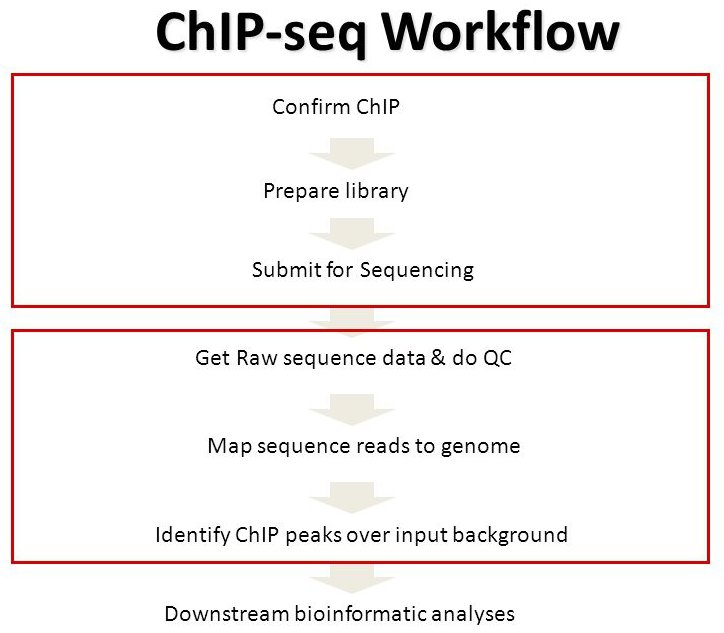
\includegraphics[width=0.7\textwidth]{c3.transcriptome/chipseq.all.01.jpg}
  \end{figure}
\end{frame}

\begin{frame}
  \frametitle{顺反组 | ChIP-Seq | 分析 | \textcolor{red}{流程}}
  \begin{figure}
    \centering
    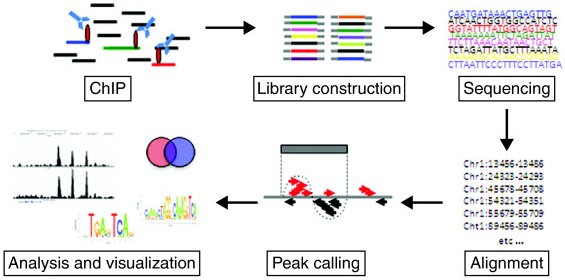
\includegraphics[width=0.9\textwidth]{c3.transcriptome/chipseq.all.02.jpg}
  \end{figure}
\end{frame}

\begin{frame}
  \frametitle{顺反组 | ChIP-Seq | 分析 | 流程}
  \begin{figure}
    \centering
    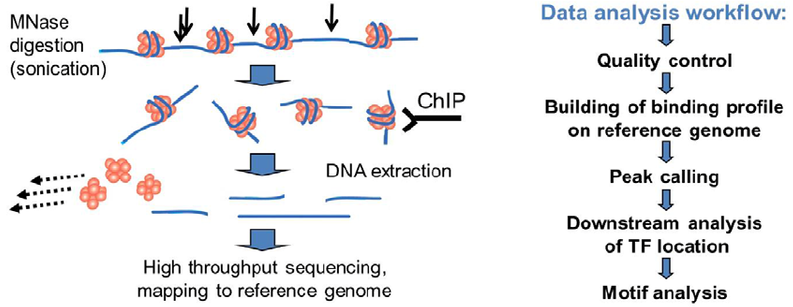
\includegraphics[width=0.9\textwidth]{c3.transcriptome/chipseq.all.03.png}
  \end{figure}
\end{frame}

\begin{frame}
  \frametitle{顺反组 | ChIP-Seq | 分析 | 流程 | \textcolor{red}{实验}}
  \begin{figure}
    \centering
    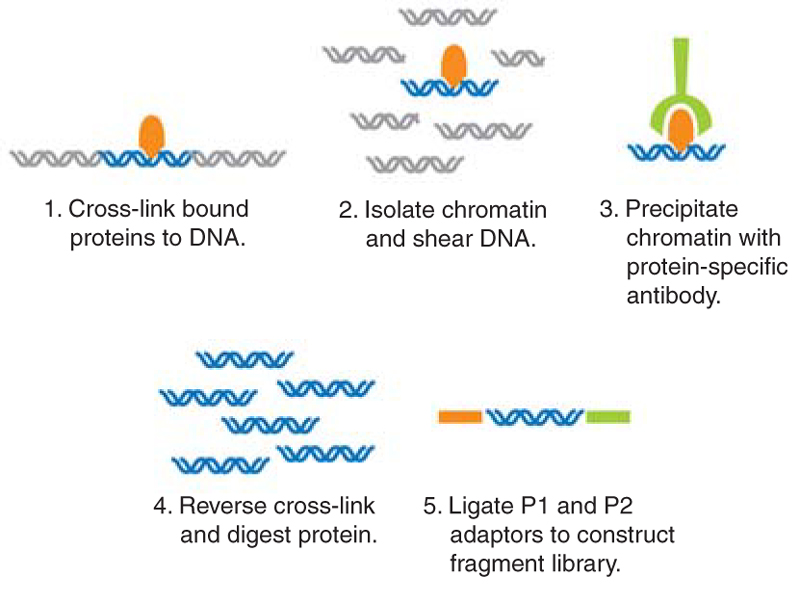
\includegraphics[width=0.8\textwidth]{c3.transcriptome/chipseq.exp.02.jpg}
  \end{figure}
\end{frame}

\begin{frame}
  \frametitle{顺反组 | ChIP-Seq | 分析 | 流程 | 实验}
  \begin{figure}
    \centering
    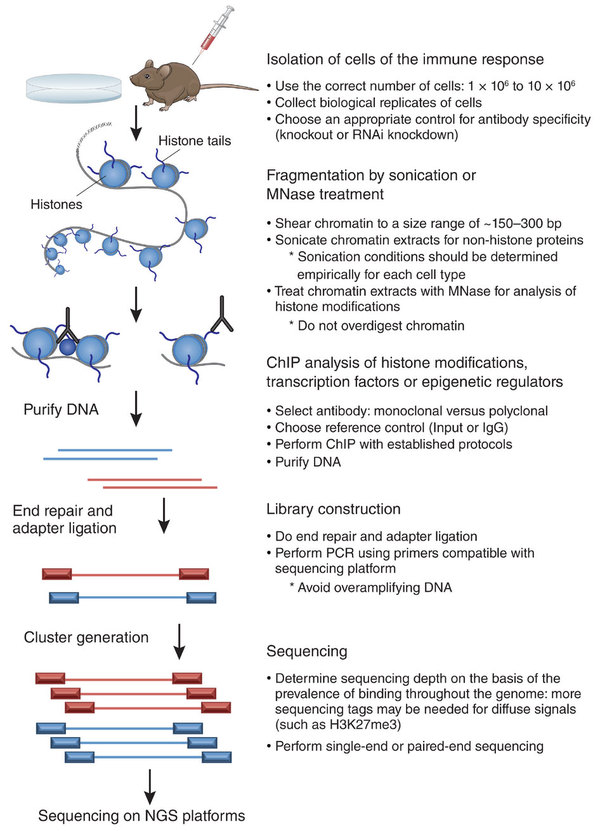
\includegraphics[width=0.46\textwidth]{c3.transcriptome/chipseq.exp.03.jpg}
  \end{figure}
\end{frame}

\begin{frame}
  \frametitle{顺反组 | ChIP-Seq | 分析 | 流程 | 实验}
  \begin{figure}
    \centering
    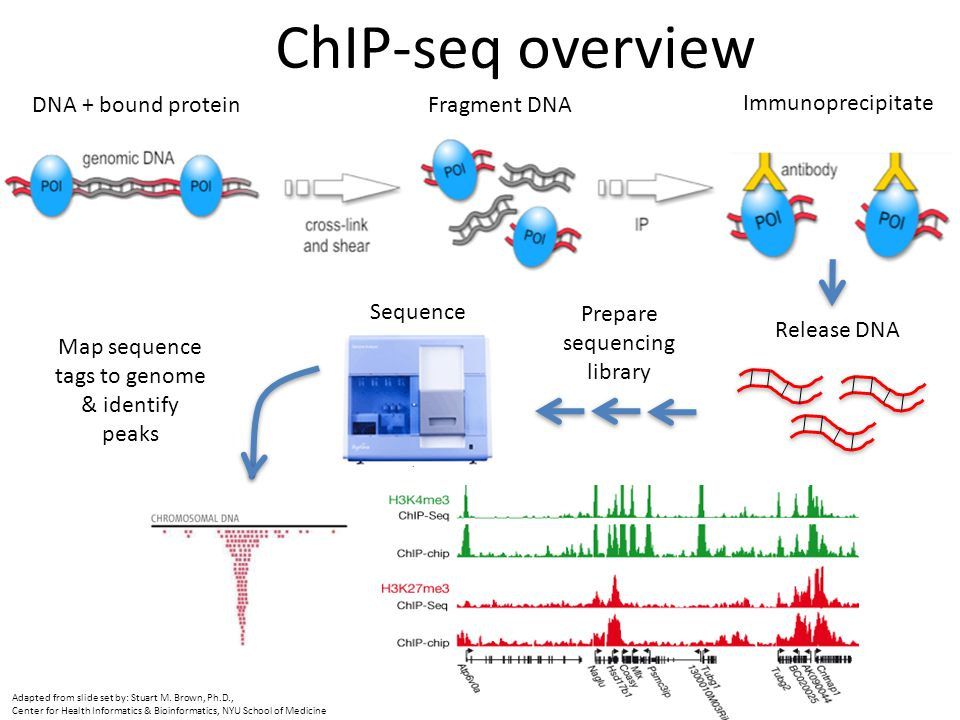
\includegraphics[width=0.8\textwidth]{c3.transcriptome/chipseq.exp.01.jpg}
  \end{figure}
\end{frame}

\begin{frame}
  \frametitle{顺反组 | ChIP-Seq | 分析 | 流程 | \textcolor{red}{生信}}
  \begin{figure}
    \centering
    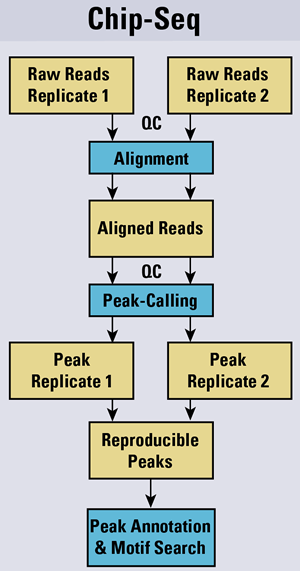
\includegraphics[width=0.33\textwidth]{c3.transcriptome/chipseq.bx.01.png}
  \end{figure}
\end{frame}

\begin{frame}
  \frametitle{顺反组 | ChIP-Seq | 分析 | 流程 | 生信}
  \begin{figure}
    \centering
    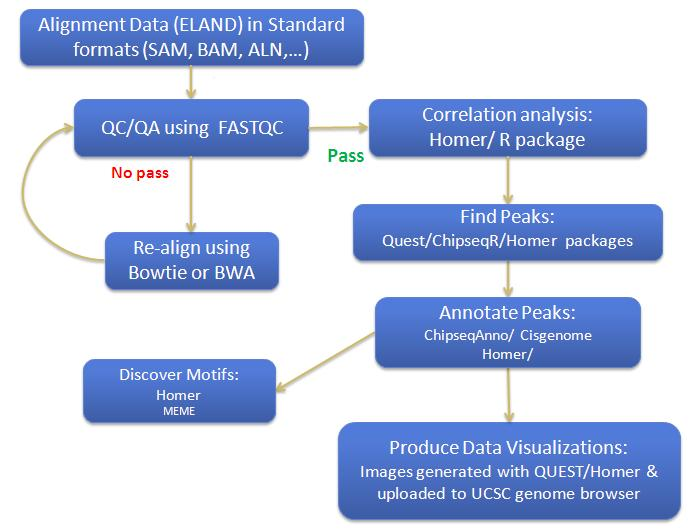
\includegraphics[width=0.8\textwidth]{c3.transcriptome/chipseq.bx.02.jpg}
  \end{figure}
\end{frame}

\begin{frame}
  \frametitle{顺反组 | ChIP-Seq | 分析 | 流程 | \textcolor{red}{生信}}
  \begin{figure}
    \centering
    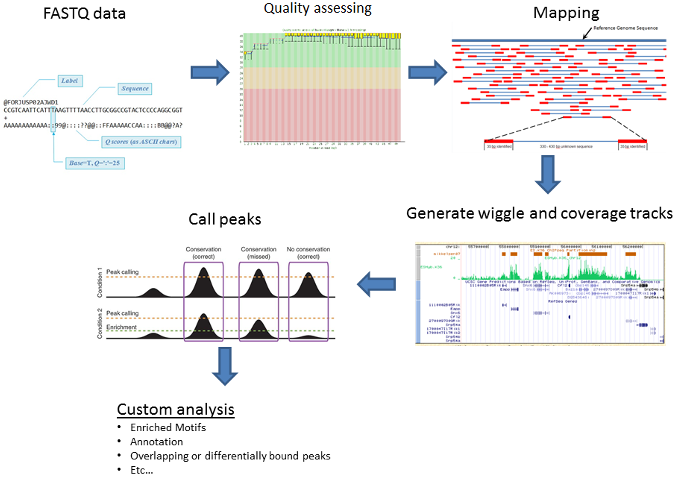
\includegraphics[width=0.9\textwidth]{c3.transcriptome/chipseq.bx.03.png}
  \end{figure}
\end{frame}

\begin{frame}
  \frametitle{顺反组 | ChIP-Seq | 分析 | 流程 | \textcolor{red}{生信}}
  \begin{figure}
    \centering
    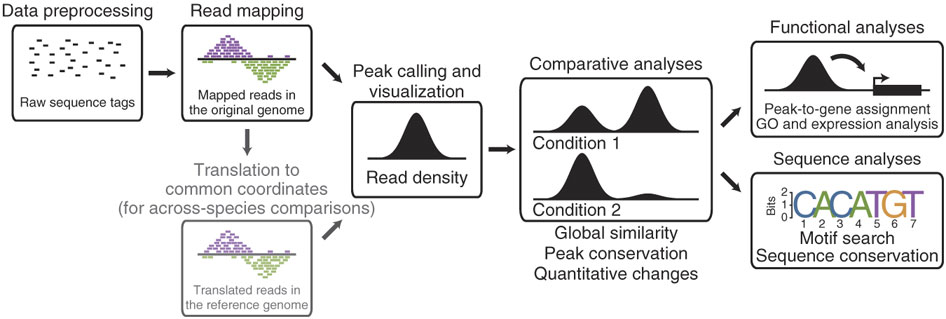
\includegraphics[width=0.9\textwidth]{c3.transcriptome/chipseq.bx.04.jpg}
  \end{figure}
\end{frame}

\begin{frame}
  \frametitle{顺反组 | ChIP-Seq | 分析 | 流程 | \textcolor{red}{生信}}
  \begin{figure}
    \centering
    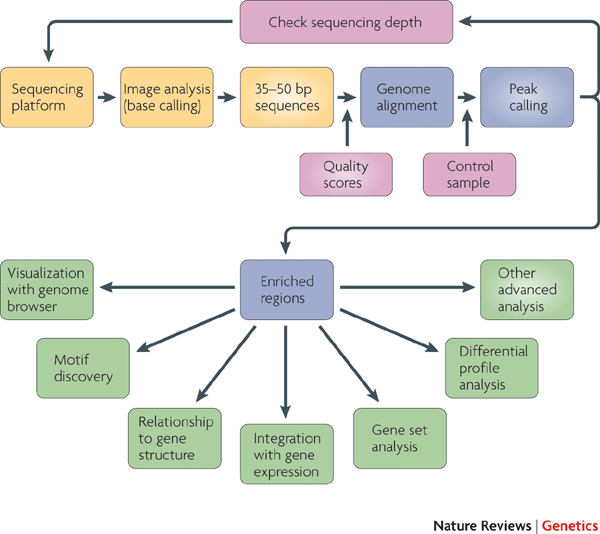
\includegraphics[width=0.75\textwidth]{c3.transcriptome/chipseq.bx.06.jpg}
  \end{figure}
\end{frame}

\begin{frame}
  \frametitle{顺反组 | ChIP-Seq | 分析 | 流程 | 生信}
  \begin{figure}
    \centering
    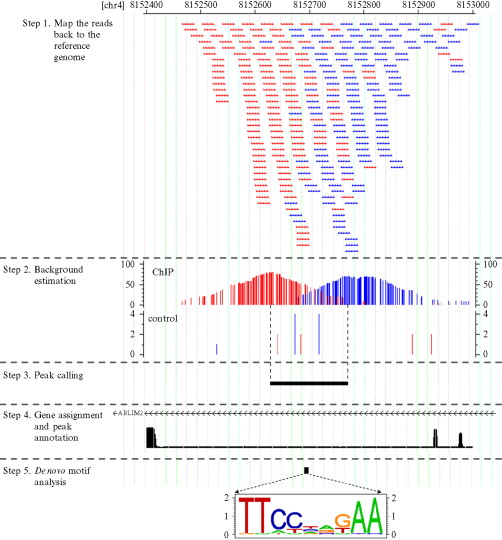
\includegraphics[width=0.6\textwidth]{c3.transcriptome/chipseq.bx.07.jpg}
  \end{figure}
\end{frame}

\begin{frame}
  \frametitle{顺反组 | ChIP-Seq | 分析 | 流程 | 生信}
  \begin{figure}
    \centering
    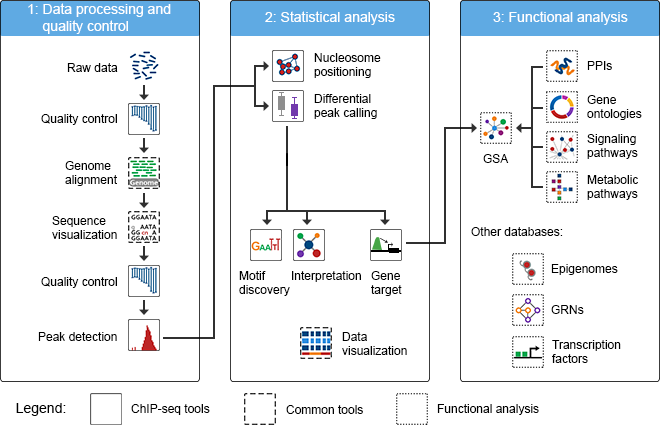
\includegraphics[width=0.9\textwidth]{c3.transcriptome/chipseq.bx.08.png}
  \end{figure}
\end{frame}

\begin{frame}
  \frametitle{顺反组 | ChIP-Seq | 分析 | 流程 | 生信}
  \begin{figure}
    \centering
    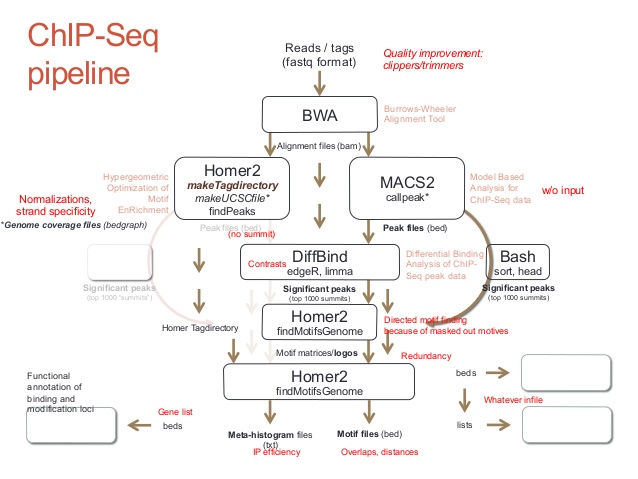
\includegraphics[width=0.85\textwidth]{c3.transcriptome/chipseq.bx.09.jpg}
  \end{figure}
\end{frame}

\begin{frame}
  \frametitle{顺反组 | ChIP-Seq | 分析 | \textcolor{red}{Peak calling}}
  \begin{block}{Peak calling}
    Peak calling是一种用于鉴定经染色质免疫沉淀-测序或MeDIP-测序实验后所得到的比对读段富集在基因组哪些区域中的一种计算方法。当免疫沉淀的蛋白质是一种转录因子时,那么DNA的富集区域就是转录因子结合位点(TFBS)。主流的Peak calling软件有MACS等。\\
    \vspace{1em}
    Peak calling可应用于转录组/外显子组测序,亦可用于对MeRIP-测序或m6A-测序的RNA表观基因组测序数据进行分析;利用如exomePeak等的软件程序,可检测出转录后的RNA修饰位点。
  \end{block}
\end{frame}

\begin{frame}
  \frametitle{顺反组 | ChIP-Seq | 分析 | Peak calling}
  {\footnotesize
  \begin{block}{Peak calling}
    Peak calling is a computational method used to identify areas in a genome that have been enriched with aligned reads as a consequence of performing a ChIP-sequencing or MeDIP-seq experiment. These areas are those where a protein interacts with DNA. When the protein is a transcription factor, the enriched area is its transcription factor binding site (TFBS). Popular software programs include MACS.\\
    \vspace{1em}
    Peak calling may be conducted on transcriptome/exome as well to RNA epigenome sequencing data from MeRIPseq or m6Aseq for detection of post-transcriptional RNA modification sites with software programs, such as exomePeak. Many of the peak calling tools are optimised for only some kind of assays such as only for transcription-factor ChIP-seq or only for DNase-seq. However new generation of peak callers such as DFilter are based on generalised optimal theory of detection and has been shown to work for nearly all kinds for tag profile signals from next-generation sequencing data. It is also possible to do more complex analysis using such tools like combining multiple ChIP-seq signal to detect regulatory sites.
  \end{block}
  }
\end{frame}

\begin{frame}
  \frametitle{顺反组 | ChIP-Seq | 分析 | \textcolor{red}{Differential peak calling}}
  {\footnotesize
  \begin{block}{Differential peak calling}
  Differential peak calling is about identifying significant differences in two ChIP-seq signals. One can distinguish between one-stage and two-stage differential peak callers.
  \end{block}
  \pause
  \begin{block}{One stage differential peak callers}
    One stage differential peak callers work in two phases: first, call peaks on individual ChIP-seq signals and second, combine individual signals and apply statistical tests to estimate differential peaks. DBChIP and MAnorm are examples for one stage differential peak callers.
  \end{block}
  \pause
  \begin{block}{Two stage differential peak callers}
 Two stage differential peak callers segment two ChIP-seq signals and identify differential peaks in one step. They take advantage of signal segmentation approaches such as Hidden Markov Models. Examples for two-stage differential peak callers are ChIPDiff, ODIN, and THOR. Differential peak calling can also be applied in the context of analyzing RNA-binding protein binding sites. 
  \end{block}
  }
\end{frame}

\begin{frame}
  \frametitle{顺反组 | ChIP-Seq | 分析 | Peak calling}
  \begin{figure}
    \centering
    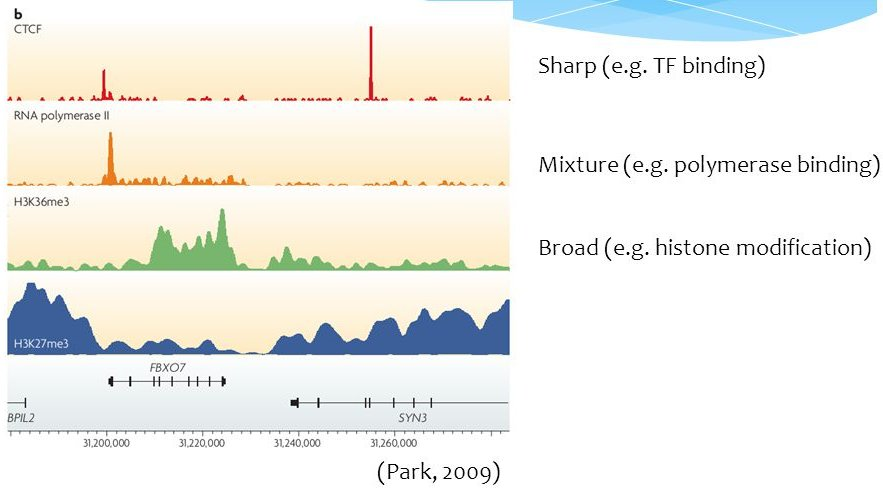
\includegraphics[width=0.9\textwidth]{c3.transcriptome/chipseq.pc.01.jpg}
  \end{figure}
\end{frame}

\begin{frame}
  \frametitle{顺反组 | ChIP-Seq | 分析 | Peak calling}
  \begin{figure}
    \centering
    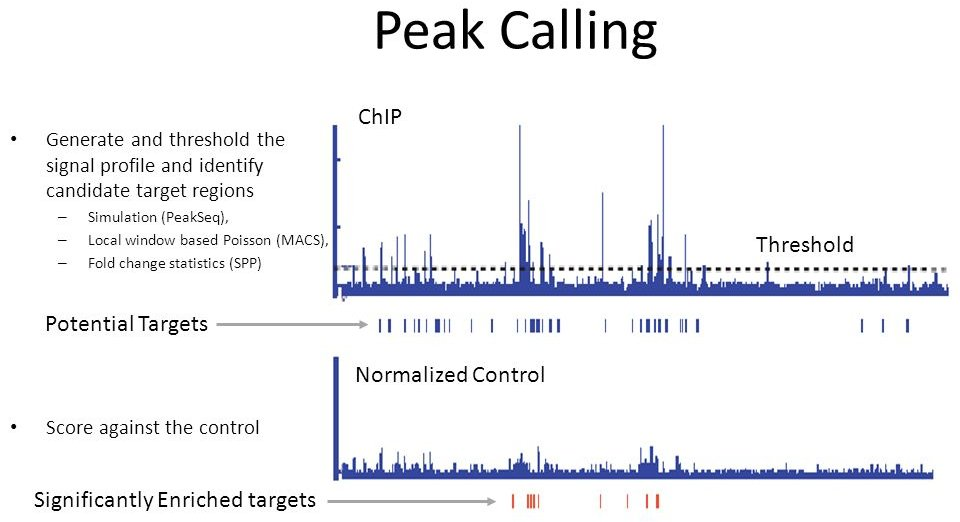
\includegraphics[width=0.9\textwidth]{c3.transcriptome/chipseq.pc.02.jpg}
  \end{figure}
\end{frame}

\begin{frame}
  \frametitle{顺反组 | ChIP-Seq | 分析 | Peak calling}
  \begin{figure}
    \centering
    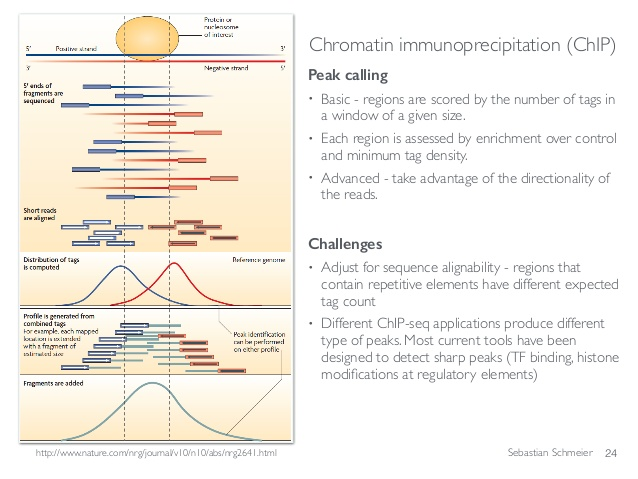
\includegraphics[width=0.48\textwidth]{c3.transcriptome/chipseq.pc.03.jpg}
  \end{figure}
\end{frame}

\begin{frame}
  \frametitle{顺反组 | ChIP-Seq | 分析 | Peak calling}
  \begin{figure}
    \centering
    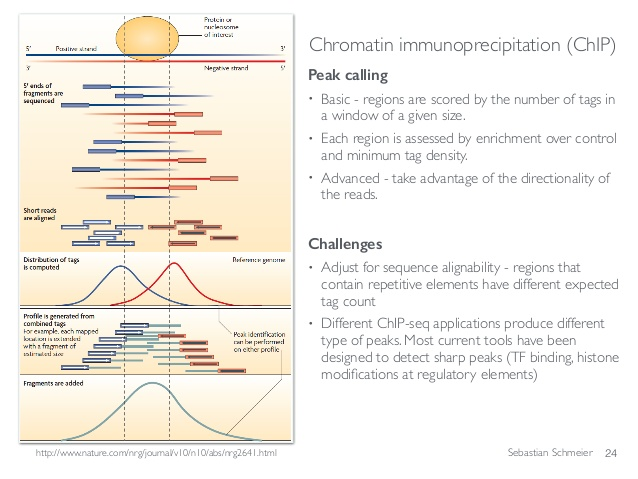
\includegraphics[width=0.9\textwidth]{c3.transcriptome/chipseq.pc.04.jpg}
  \end{figure}
\end{frame}

\begin{frame}
  \frametitle{顺反组 | ChIP-Seq | 分析 | \textcolor{red}{应用}}
  \begin{figure}
    \centering
    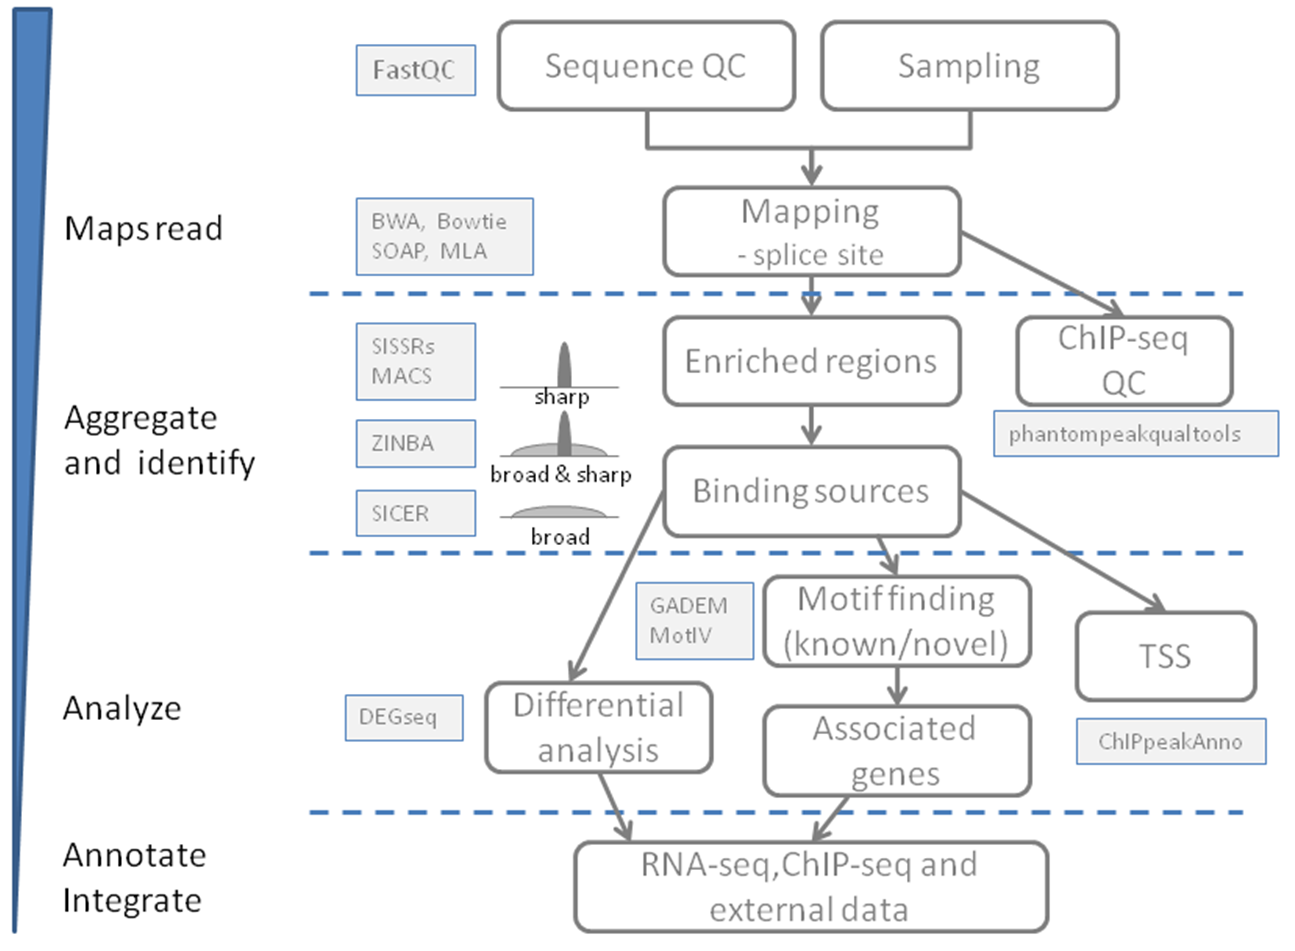
\includegraphics[width=0.8\textwidth]{c3.transcriptome/chipseq.seqs.01.png}
  \end{figure}
\end{frame}

\begin{frame}
  \frametitle{顺反组 | ChIP-Seq | 分析 | 应用}
  \begin{figure}
    \centering
    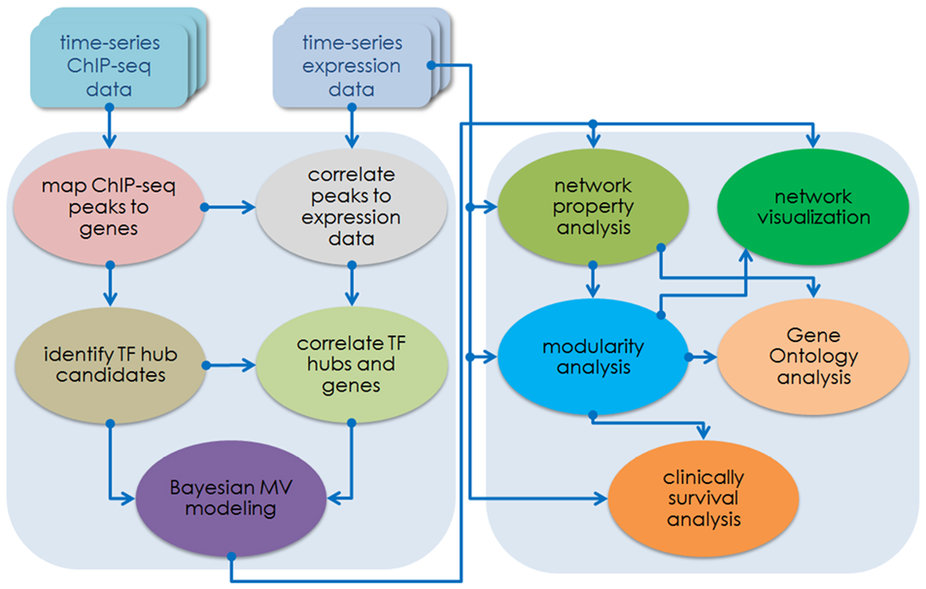
\includegraphics[width=0.9\textwidth]{c3.transcriptome/chipseq.seqs.02.jpg}
  \end{figure}
\end{frame}

\begin{frame}
  \frametitle{顺反组 | ChIP-Seq | 分析 | 应用}
  \begin{figure}
    \centering
    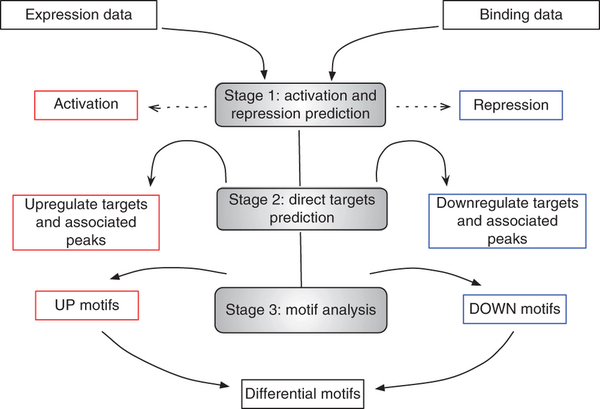
\includegraphics[width=0.9\textwidth]{c3.transcriptome/chipseq.seqs.03.jpg}
  \end{figure}
\end{frame}

\begin{frame}
  \frametitle{顺反组 | ChIP-Seq | 分析 | \textcolor{red}{工具}}
  \begin{figure}
    \centering
    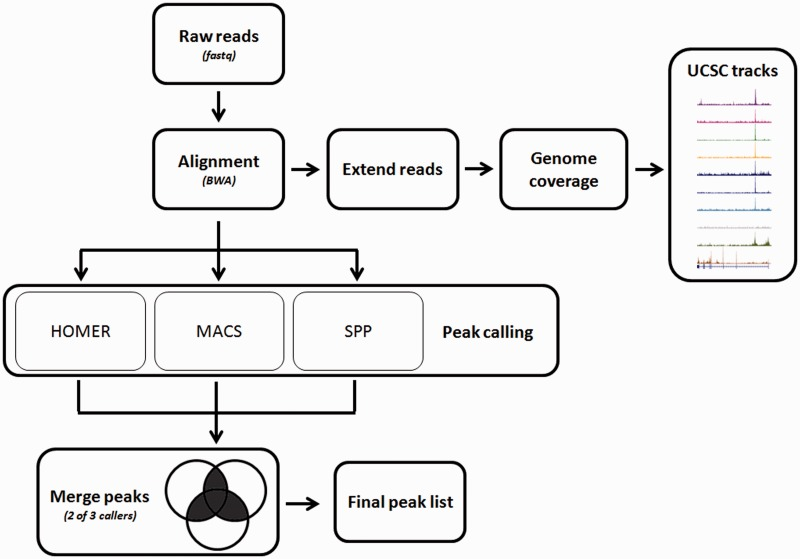
\includegraphics[width=0.9\textwidth]{c3.transcriptome/chipseq.tools.01.jpg}
  \end{figure}
\end{frame}

\begin{frame}
  \frametitle{顺反组 | ChIP-Seq | 分析 | \textcolor{red}{工具}}
  \begin{block}{MACS}
    Model-based Analysis of ChIP-Seq (MACS) empirically models the length of the sequenced ChIP fragments, which tends to be shorter than sonication or library construction size estimates, and uses it to improve the spatial resolution of predicted binding sites. MACS also uses a dynamic Poisson distribution to effectively capture local biases in the genome sequence, allowing for more sensitive and robust prediction. MACS compares favorably to existing ChIP-Seq peak-finding algorithms, is publicly available open source, and can be used for ChIP-Seq with or without control samples.
  \end{block}
\end{frame}

\begin{frame}
  \frametitle{顺反组 | ChIP-Seq | 分析 | 工具}
  \begin{block}{PeakSeq}
    PeakSeq is a program for identifying and ranking peak regions in ChIP-Seq experiments. It takes as input, mapped reads from a ChIP-Seq experiment, mapped reads from a control experiment and outputs a file with peak regions ranked with increasing Q-values. 
  \end{block}
\end{frame}

\begin{frame}
  \frametitle{顺反组 | ChIP-Seq | 分析 | 工具}
  \begin{block}{HOMER}
    HOMER (Hypergeometric Optimization of Motif EnRichment) is a suite of tools for Motif Discovery and next-gen sequencing analysis.  It is a collection of command line programs for unix-style operating systems written in Perl and C++. HOMER was primarily written as a \textit{de novo} motif discovery algorithm and is well suited for finding 8-20 bp motifs in large scale genomics data.  HOMER contains many useful tools for analyzing ChIP-Seq, GRO-Seq, RNA-Seq, DNase-Seq, Hi-C and numerous other types of functional genomics sequencing data sets.
  \end{block}
\end{frame}

\begin{frame}
  \frametitle{顺反组 | ChIP-Seq | 分析 | 工具 | MACS}
  \begin{figure}
    \centering
    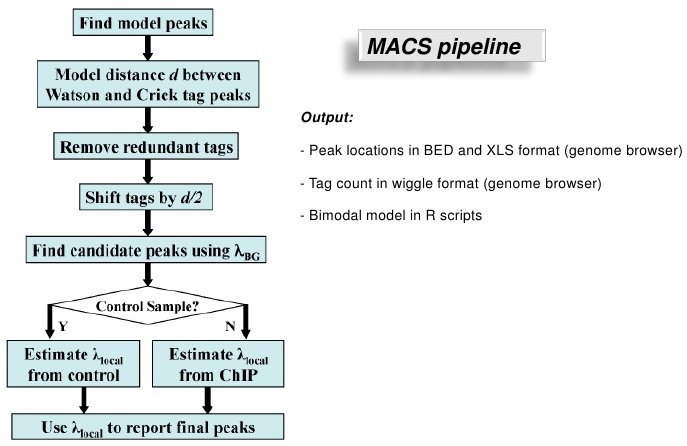
\includegraphics[width=0.9\textwidth]{c3.transcriptome/chipseq.macs.01.jpg}
  \end{figure}
\end{frame}

\begin{frame}
  \frametitle{顺反组 | ChIP-Seq | 分析 | 工具 | MACS}
  \begin{figure}
    \centering
    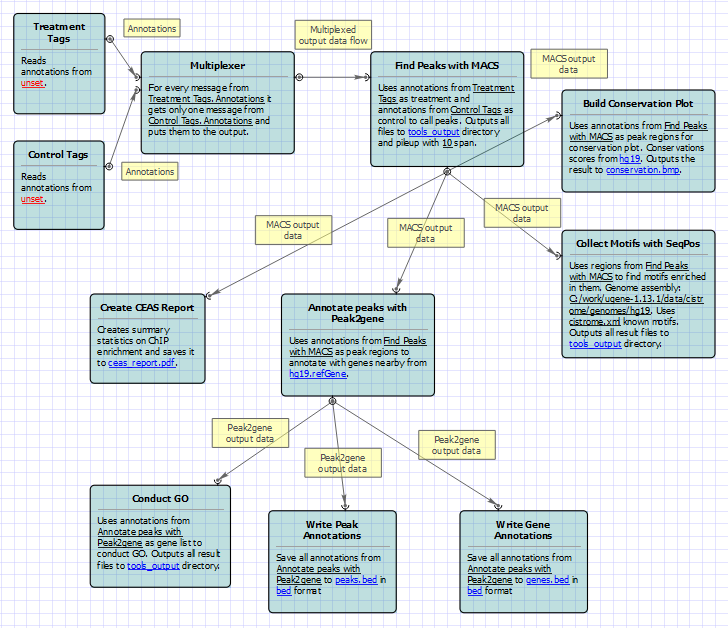
\includegraphics[width=0.75\textwidth]{c3.transcriptome/chipseq.macs.02.png}
  \end{figure}
\end{frame}

\begin{frame}
  \frametitle{顺反组 | ChIP-Seq | 分析 | 工具 | \textcolor{red}{注释}}
  \begin{figure}
    \centering
    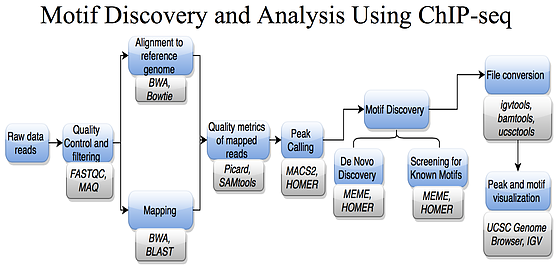
\includegraphics[width=0.9\textwidth]{c3.transcriptome/chipseq.bx.00.png}
  \end{figure}
\end{frame}

\begin{frame}
  \frametitle{顺反组 | ChIP-Seq | 分析 | 工具 | 注释}
  \begin{figure}
    \centering
    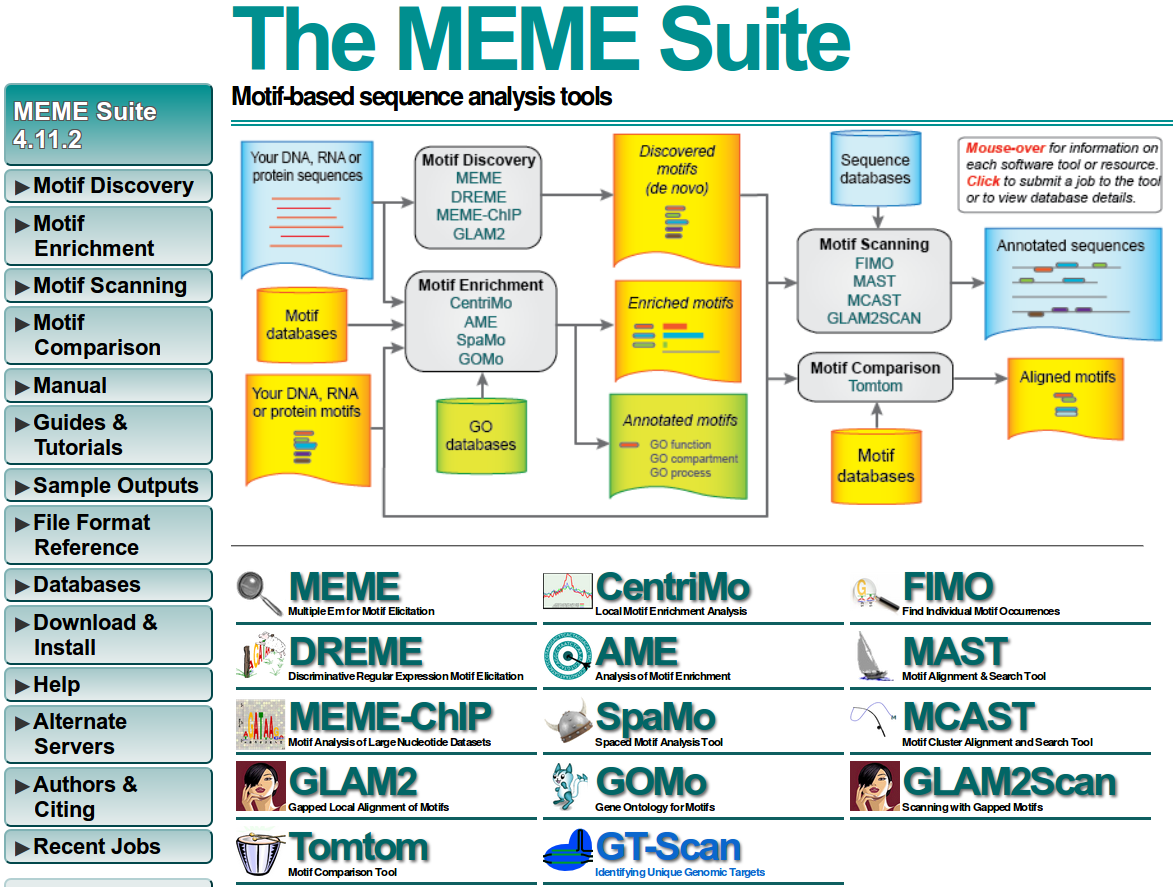
\includegraphics[width=0.85\textwidth]{c3.transcriptome/chipseq.meme.01.png}
  \end{figure}
\end{frame}

\subsubsection{应用实例}
\begin{frame}
  \frametitle{顺反组 | ChIP-Seq | 实例}
  {\footnotesize
    \begin{block}{Nature Methods, 2007}
  STAT1 DNA association: ChIP-seq was used to study STAT1 targets in HeLA S3 cells. The performance of ChIP-seq was then compared to the alternative protein–DNA interaction methods of ChIP-PCR and ChIP-chip.\\
  \vspace{0.5em}
  ChIP-seq offers an alternative to ChIP-chip. STAT1 experimental ChIP-seq data have a high degree of similarity to results obtained by ChIP-chip for the same type of experiment, with >64\% of peaks in shared genomic regions. Because the data are sequence reads, ChIP-seq offers a rapid analysis pipeline (as long as a high-quality genome sequence is available for read mapping, and the genome doesn't have repetitive content that confuses the mapping process) as well as the potential to detect mutations in binding-site sequences, which may directly support any observed changes in protein binding and gene regulation.\\
  \vspace{0.5em}
  Robertson G et al.(2007) Genome-wide profiles of STAT1 DNA association using chromatin immunoprecipitation and massively parallel sequencing. Nature Methods 4: 651–657.
    \end{block}
}
\end{frame}

\begin{frame}
  \frametitle{顺反组 | ChIP-Seq | 实例}
  \begin{figure}
    \centering
    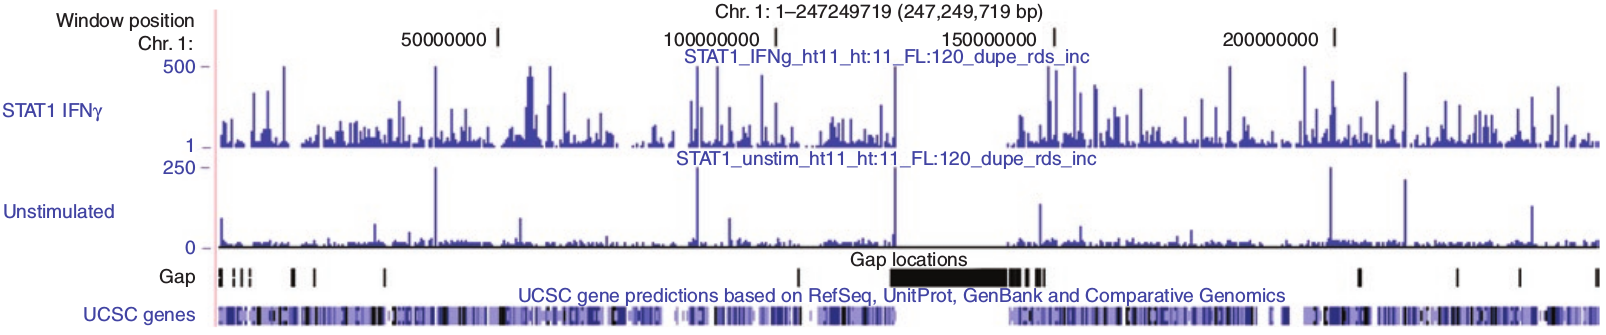
\includegraphics[width=\textwidth]{c3.transcriptome/chipseq.example.01.png}
  \end{figure}
\end{frame}

\begin{frame}
  \frametitle{顺反组 | ChIP-Seq | 实例}
  \begin{block}{Cell, 2007}
  Nucleosome Architecture of Promoters: Using ChIP-seq, it was determined that Yeast genes seem to have a minimal nucleosome-free promoter region of 150bp in which RNA polymerase can initiate transcription.\\
  \vspace{0.5em}
  Schmid et al. (2007) ChIP-Seq Data reveal nucleosome architecture of human promoters. Cell 131: 831–832
  \end{block}
\end{frame}

\begin{frame}
  \frametitle{顺反组 | ChIP-Seq | 实例}
  \begin{figure}
    \centering
    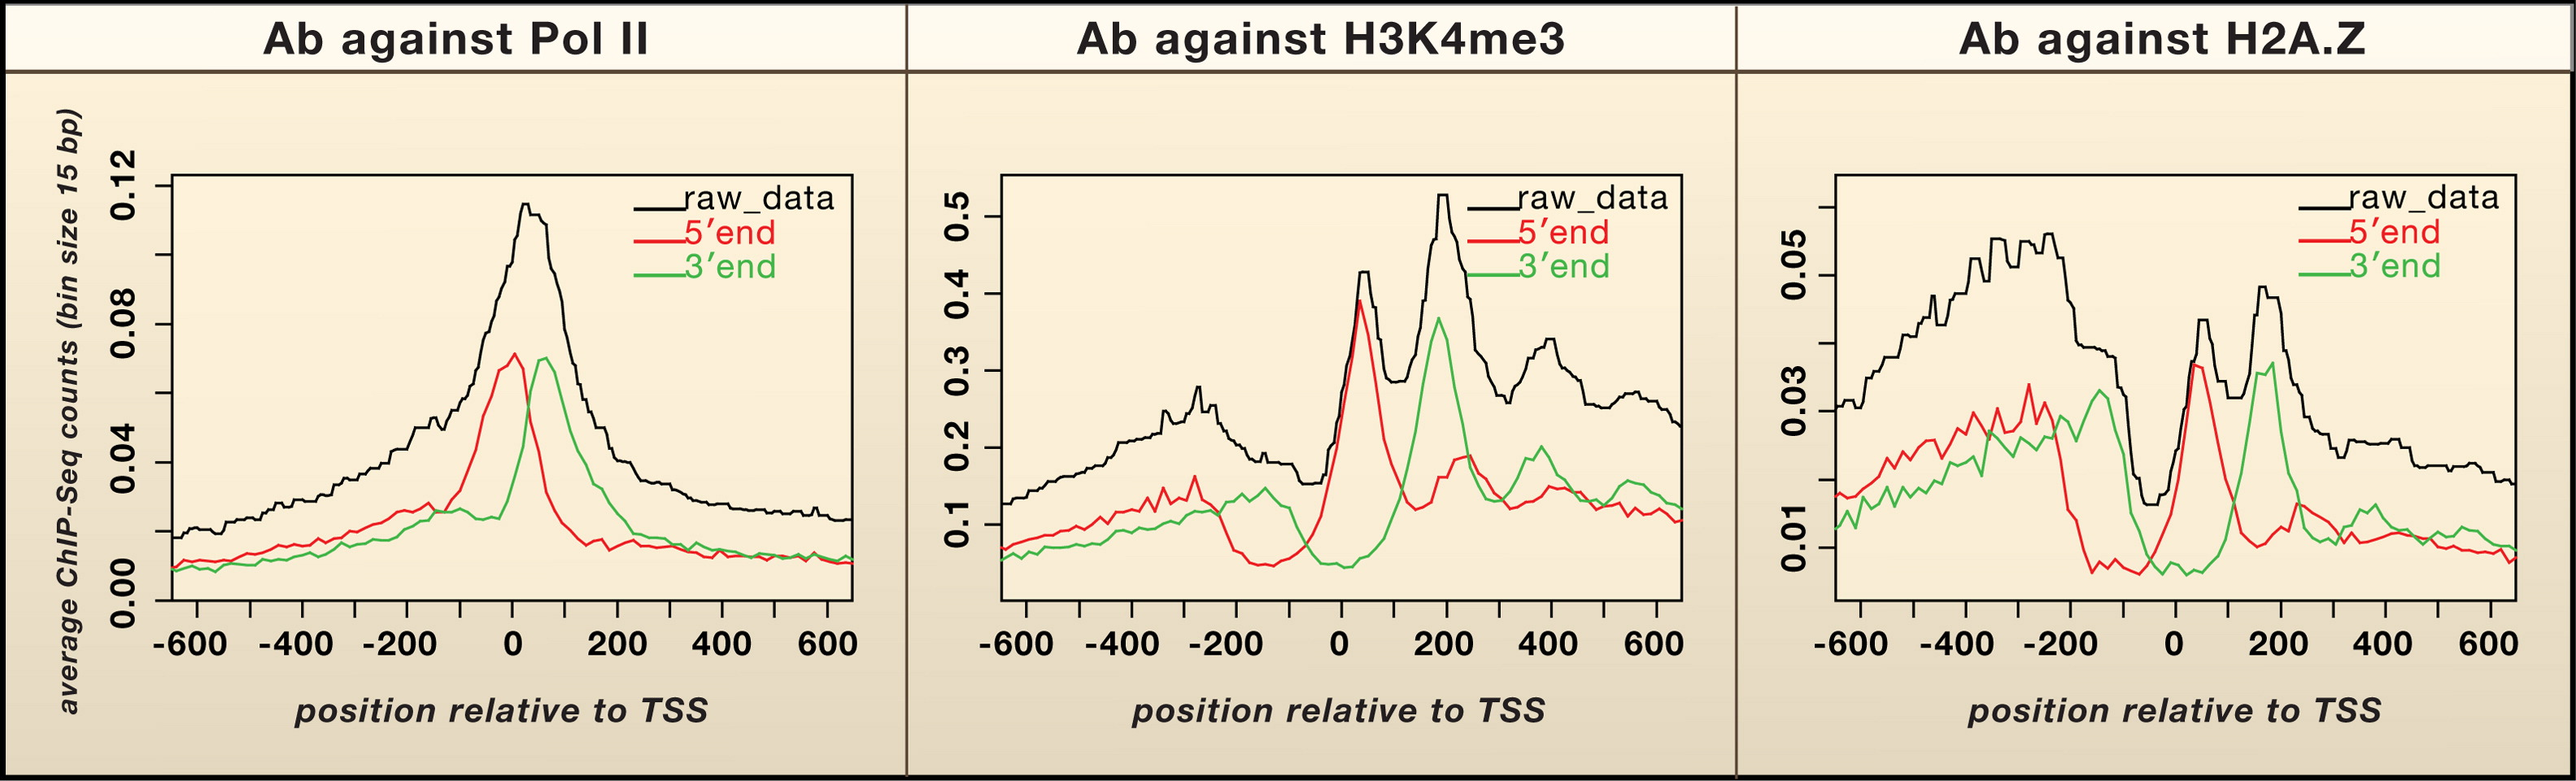
\includegraphics[width=\textwidth]{c3.transcriptome/chipseq.example.02.jpg}
  \end{figure}
\end{frame}

\begin{frame}
  \frametitle{顺反组 | ChIP-Seq | 实例}
  \begin{block}{Nature Genetics, 2010}
  Transcription factor conservation: ChIP-seq was used to compare conservation of TFs in the forebrain and heart tissue in embryonic mice. The authors identified and validated the heart functionality of transcription enhancers, and determined that transcription enhancers for the heart are less conserved than those for the forebrain during the same developmental stage.\\
  \vspace{0.5em}
  Blow, M. J., McCulley, D. J., Li, Z., Zhang, T., Akiyama, J. A., Holt, A., Plajzer-Frick, I., Shoukry, M., Wright, C., Chen, F., Afzal, V., Bristow, J., Ren, B., Black, B. L., Rubin, E. M., Visel, A., \& Pennacchio, L. A. (2010). ChIP-seq identification of weakly conserved heart enhancers. Nature Genetics, 42, 806-810.
  \end{block}
\end{frame}

\begin{frame}
  \frametitle{顺反组 | ChIP-Seq | 实例}
  \begin{figure}
    \centering
    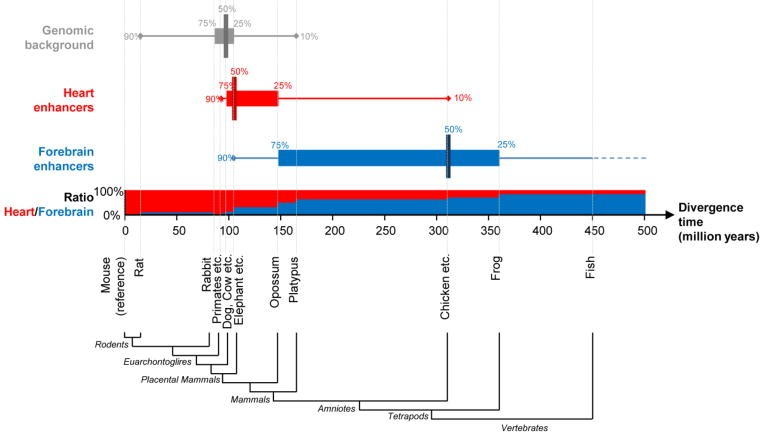
\includegraphics[width=\textwidth]{c3.transcriptome/chipseq.example.03.jpg}
  \end{figure}
\end{frame}

\begin{frame}
  \frametitle{顺反组 | ChIP-Seq | 实例}
  {\footnotesize
  \begin{block}{Genome Research, 2011}
  Genome-wide ChIP-seq: ChIP-sequencing was completed on the worm C. elegans to explore genome-wide binding sites of 22 transcription factors. Up to 20\% of the annotated candidate genes were assigned to transcription factors. Several transcription factors were assigned to non-coding RNA regions and may be subject to developmental or environmental variables. The functions of some of the transcription factors were also identified. Some of the transcription factors regulate genes that control other transcription factors. These genes are not regulated by other factors. Most transcription factors serve as both targets and regulators of other factors, demonstrating a network of regulation.\\
  \vspace{0.5em}
  Niu, W., Lu, Z. J., Zhong, M., Sarov, M., Murray, J. I., Brdlik, C. M., Janette, J., Chen, C., Alves, P., Preston, E., Slightham, C., Jiang, L., Hyman, A. A., Kim. S. K., Waterston, R. H., Gerstein, M., Snyder, M., \& Reinke, V. (2011). Diverse transcription factor binding features revealed by genome-wide ChIP-seq in C. elegans. Genome Research, 21, 245-254.
  \end{block}
}
\end{frame}

\begin{frame}
  \frametitle{顺反组 | ChIP-Seq | 实例}
  \begin{figure}
    \centering
    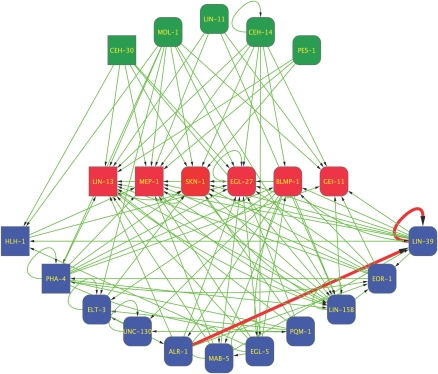
\includegraphics[width=0.7\textwidth]{c3.transcriptome/chipseq.example.04.jpg}
  \end{figure}
\end{frame}

\begin{frame}
  \frametitle{顺反组 | ChIP-Seq | 实例}
  \begin{block}{Nature Biotechnology, 2013}
  Inferring regulatory network: ChIP-seq signal of Histone modification were shown to be more correlated with transcription factor motifs at promoters in comparison to RNA level. Hence author proposed that using histone modification ChIP-seq would provide more reliable inference of gene-regulatory networks in comparison to other methods based on expression.\\
  \vspace{0.5em}
  Vibhor Kumar, Masafumi Muratani, Nirmala Arul Rayan, Petra Kraus, Thomas Lufkin, Huck Hui Ng and Shyam Prabhakar. Uniform, optimal signal processing of mapped deep-sequencing data. Nature biotechnology, 2013.
  \end{block}
\end{frame}

\begin{frame}
  \frametitle{顺反组 | ChIP-Seq | 实例}
  \begin{figure}
    \centering
    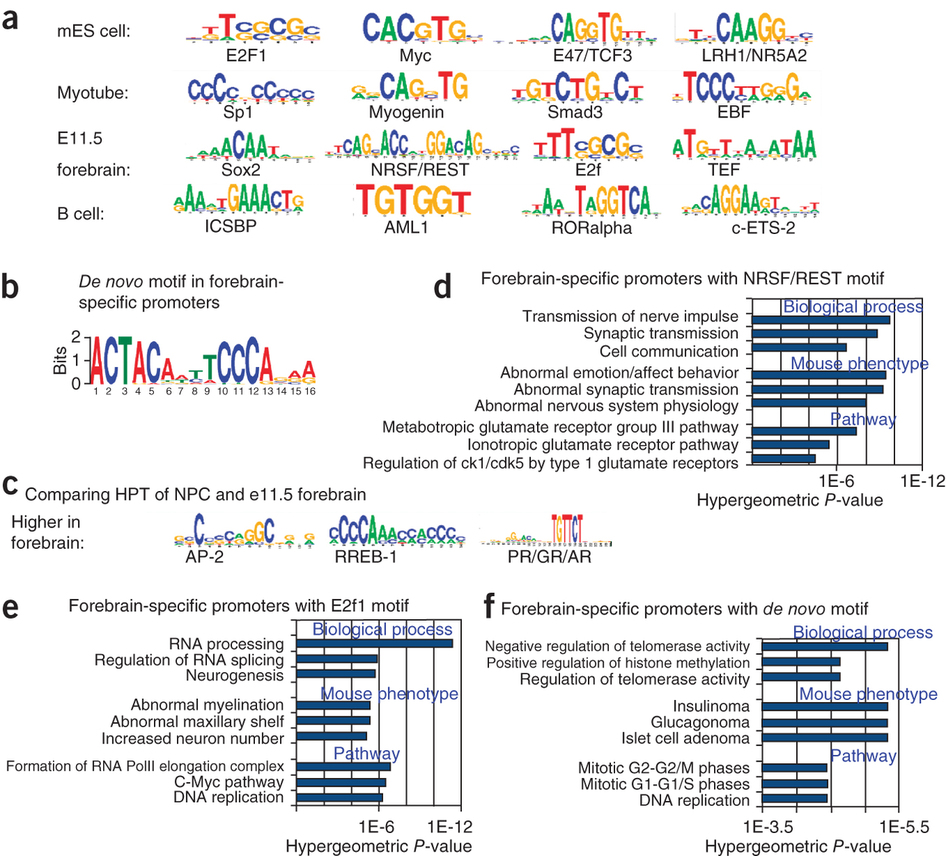
\includegraphics[width=0.7\textwidth]{c3.transcriptome/chipseq.example.05.jpg}
  \end{figure}
\end{frame}

